% !TEX root = ./main_TCS.tex


\section{From Reaction Systems to c\CNA}
\label{sec:trans}
Here we define an encoding of
%a translation from 
Reaction Systems into c\CNA.
The idea is to define separated processes for representing the behaviour of each entity, each reaction, 
and for the provisioning of each entity by the context.

In the following we refer to a given set of entities $S$ and a set of reactions $A \subseteq \mathit{rac}(S)$, i.e. that the Reaction System ${\cal A} = (S, A)$ is known.

\paragraph{Processes for entities}
Given an entity $s \in S$, we exploit five different pairs of channel names for the interactions over $s$:
\begin{itemize}
\item names $s_i$, $s_o$ are used to test the presence of $s$ in the system; 
\item names $\widehat{s}_i$, $\widehat{s}_o$ are used to test the provisioning of $s$ from the context;
\item names $\widetilde{s}_i$, $\widetilde{s}_o$  are used to test the production of $s$ by some reaction; 
\item names $\overline{s}_i$, $\overline{s}_o$ are used to test the absence of $s$ in the system; 
\item  names $\underline{s}_i$, $\underline{s}_o$ are used to test the absence of $s$ from the context.
\end{itemize}
We let $P_s$ be the process implementing the  presence of $s$ in the system, and $\overline{P_s}$ be the one for its absence.
They can be seen as instances of the same template, which is given below. 

\[
\begin{array}{lcl@{\hskip 1cm}lcl}
 P_s &\defeq & E(s,\widetilde{s},\widehat{s},\underline{s}) 
 &
 \overline{P_s}& \defeq & E(\overline{s},\widetilde{s},\widehat{s},\underline{s})
\end{array}
\]
%{\color{red}
%\[
%\begin{array}{rcl}
% P(s,\tilde{s},\hat{s},\underline{s}) & \defeq &\sum_{h_j,k_j\in\{0,1\}}
%  (\startchain{s_i}\chainedlink{s_o}{\noact}\chainend{\noact})^{h_j} \ (\startchain{\tilde{s}_i}\chainedlink{\tilde{s}_o}{\noact}\chainend{\noact})^{k_j}\ \link{\hat{s}_i}{\hat{s}_o}.P_s\\
%&&\ + \\
%&&
%\sum_{\scriptsize \begin{array}{l}h_j,k_j, \\ h'_j\in\{0,1\}\end{array}}
%  (\startchain{s_i}\chainedlink{s_o}{\noact}\chainend{\noact})^{h_j} \ (\startchain{\tilde{s}_i}\chainedlink{\tilde{s}_o}{\noact}\chainend{\noact})^{k_j} \  \startchain{\tilde{s}_i}\chainedlink{\tilde{s}_o}{\noact}\chainend{\noact} \    (\startchain{s_i}\chainedlink{s_o}{\noact}\chainend{\noact})^{h'_j} \ \link{\underline{s}_i}{\underline{s}_o}.P_s \\
%
%%\sum_{R_1+R_2\geq 0}(\sum_{h,k \in[0,1]} 
%%  (\startchain{s_i}\chainedlink{s_o}{\noact}\chainend{\noact})^h \ (\startchain{\tilde{s}_i}\chainedlink{\tilde{s}_o}{\noact}\chainend{\noact})^k)^{R_1} \startchain{\tilde{s}_i}\chainedlink{\tilde{s}_o}{\noact}\chainend{\noact} (\sum_{h ,k\in[0,1]}
%%  (\startchain{s_i}\chainedlink{s_o}{\noact}\chainend{\noact})^h \ (\startchain{\tilde{s}_i}\chainedlink{\tilde{s}_o}{\noact}\chainend{\noact})^k)^{R_2} \link{\underline{s}_i}{\underline{s}_o}.P_s\\
%&&\ +\\
%&&\sum_{j\geq 0}(
%  \startchain{s_i}\chainedlink{s_o}{\noact}\chainend{\noact})^j\ \ \link{\underline{s}_i}{\underline{s}_o}.\overline{P_s}
%\end{array}
%\]
%}
\[
\begin{array}{rcl}
 E(s,\widetilde{s},\widehat{s},\underline{s}) & \defeq &\sum_{h,k\geq 0}  
  (\startchain{s_i}\chainedlink{s_o}{\noact}\chainend{\noact})^h \ \startchain{\widehat{s}_i}\chainedlink{\widehat{s}_o}{\noact}\chainend{\noact} (\startchain{\widetilde{s}_i}\chainedlink{\widetilde{s}_o}{\noact}\chainend{\noact})^k.P_s\\
&&\ + \\
&&
\sum_{h\geq 0,k\geq 1}
 (\startchain{s_i}\chainedlink{s_o}{\noact}\chainend{\noact})^h \ \startchain{\underline{s}_i}\chainedlink{\underline{s}_o}{\noact}\chainend{\noact}(\startchain{\widetilde{s}_i}\chainedlink{\widetilde{s}_o}{\noact}\chainend{\noact})^k.P_s\\
&&\ +\\
&&\sum_{h\geq 0}(\startchain{s_i}\chainedlink{s_o}{\noact}\chainend{\noact})^h \ \link{\underline{s}_i}{\underline{s}_o}.\overline{P_s}
\end{array}
\]

The first line of $ E(s,\widetilde{s},\widehat{s},\underline{s})$ accounts for the case where $s$ is tested for presence by $h$ reactions and produced by $k$ reactions, while being provided by the context ($\link{\widehat{s}_i}{\widehat{s}_o}$).
Thus, $s$ will be present at the next step (the continuation is $P_s$). Here $h$ and $k$ are not known a priori and therefore any
combination is possible. 
In practice, by knowing the number of reactions that test $s$, we can bound the maximum 
values of $h$ and $k$.
The second line accounts for the analogous case where $s$ is not provided by the context ($\link{\underline{s}_i}{\underline{s}_o}$). 
The condition $k\geq 1$ guarantees that $s$ will remain present (the continuation is $P_s$).
%Here taking
%$h = \sum_{j\geq0} h_j +h'_j$, $k = (\sum_{j \geq 0} k_j )  + 1$ guarantees that $s$ will be present in the next step. Please note that 
The third line accounts for the case where $s$ is tested for presence, but it is neither produced nor provided by  the context. Therefore, in the next step $s$ will be absent in the system (the continuation is $\overline{P_s}$).
Note that in the case of $\overline{P_s}$ the test for presence of $s$ in the system is just replaced by the test for its absence.
%Process $P_s$ (and $\overline{P_s}$) offers link chain prefixes for all the possible
% permutations of the solid links; nevertheless if the reactions, and their enumeration, is known
% the code of $P_s$ can be drastically simplified.

\paragraph{Processes for reactions}
We assume that all the reactions $a$ are numbered and use $j$ as an index for reactions.
We introduce two channel names for each reaction $aj$:
\begin{itemize}
\item $r_j$ to mark the occurrence of the reaction;
\item $p_j$ to mark the product set of the reaction.
\end{itemize}
We shall exploit names $r_j,p_j$ to join the chains provided by the application of all the reactions. 
%each reaction $a$ is 
%assigned a progressive number $j$.
The process for the $j$th reaction $aj=(R_j,I_j,P_j)$ must assert either the possibility to apply the reaction or its impossibility.
The first case happens when all its reactants are present (the link $\link{s_i}{s_o}$ is requested for any $s\in R_j$) and all its inhibitors are absent (the link $\link{\overline{e}_i}{\overline{e}_o}$ is requested for any $e\in I_j$), then the product set is released (the link $\link{\widetilde{c}_i}{\widetilde{c}_o}$ is requested for any $c\in P_j$).
The second case can happen for two reasons: one of the reactants is absent (the link $\link{\overline{s}_i}{\overline{s}_o}$ is requested for some $s\in R_j$) or one of the inhibitors is present (the link $\link{e_i}{e_o}$ is requested for some $e\in I_j$).
The process is recursive so that reactions can be applied at any step.
\[
\begin{array}{lcl@{\quad}l}
P_{aj} \defeq \\ 
 ^{r_j} \backslash  \blockchain{s_i}{s_o}{s \in R_j} \link{}{} \blockchain{\overline{e}_i}{\overline{e}_o}{e \in I_j} \chainedlink{r_{j+1}}{\noact}\chainedlink{\noact}{p_j}\link{}{} \blockchain{\widetilde{c}_i}{\widetilde{c}_o}{c \in P_j} \backslash_{p_{j+1}}.P_{aj} & \mbox{\small  \{$aj$ is applicable\}}\\
 + \ \\
 \sum_{s\in R_j}\startchain{r_j}\chainedlink{\overline{s}_i}{\noact}\chainedlink{\noact}{\overline{s}_o} \chainedlink{r_{j+1}}{\noact}\chainedlink{\noact}{p_{j}}\chainend{p_{j+1}}.P_{aj}  & \mbox{\small  \{$aj$ is not applicable\}}\\
+\\
 \sum_{e\in I_j}\startchain{r_j}\chainedlink{e_i}{\noact} \chainedlink{\noact}{e_o} \chainedlink{r_{i+1}}{\noact}\chainedlink{\noact}{p_{j}}\chainend{p_{j+1}}.P_{aj}  & \mbox{\small \{$aj$ is not applicable\}}\\
\end{array}
\]

Channels $r_j$ and $r_{j+1}$ enclose the enabling/disabling condition of reaction $aj$.
Channels $p_j$ and $p_{j+1}$ enclose the links related to the entities produced by $aj$.
We will see that all the link chain labels of transitions follow the same schema: first we find all the reactions limited to the reactants and inhibitors (chained using $r_j$ channels), then all the supplies by the contexts (chained using the channel $\mathit{cxt}$, to be introduced next), and finally the products for all the reactions (chained using $p_j$ channels). 
For notational convenience, we fix that 
%$r_1 = \silent$,
$r_{|A|+1} = \mathit{cxt}$ and $p_{|A|+1}=\silent$.
{\color{red} Please, recall that $A$ is a subset of reactions in $S$.}
In the following there is an example explaining this schema.
%\[
%\begin{array}{lcl@{\qquad}l}
%P_{aj}& \defeq & 
% ^{r_j} \backslash  \blockchain{s_i}{s_o}{s \in R_j} \, \link{}{} \blockchain{\overline{e}_i}{\overline{e}_o}{e \in I_j} \, \link{}{}
% \blockchain{\tilde{c}_i}{\tilde{c}_o}{c \in P_j}\, \backslash_{r_{j+1}}.P_{aj} & \mbox{\small  \{$aj$ is applicable\}}\\
%&& + \ \\
%&& \sum_{s\in R_j}\startchain{r_j}\chainedlink{\overline{s}_i}{\noact}\chainedlink{\noact}{\overline{s}_o} \chainend{r_{j+1}}.P_{aj}  & \mbox{\small  \{$aj$ is not applicable\}}\\
%&&+\\
%&& \sum_{e\in I_j}\startchain{r_j}\chainedlink{e_i}{\noact} \chainedlink{\noact}{e_o} \chainend{r_{i+1}}.P_{aj}  & \mbox{\small \{$aj$ is not applicable\}}\\
%\end{array}
%\]

\paragraph{Processes for contexts}
For marking the part of the chain provided by the context, we exploit the name $\mathit{cxt}$.
In RSs, the context sequence $\gamma$ provides a set of entities $C_n$ at each instant of time $n$: for each entity $s \in S$, the context must say if the entity is provided or not.
Correspondingly, we introduce another process $\mathit{Cxt}_n$ defined as follows:
\[
\begin{array}{lcl}
\mathit{Cxt}_n &\defeq &
%\left \{
^{cxt} \backslash  \blockchain{\hat{s}_i}{\hat{s}_o}{s\!\in \!C_n}  \link{}{} \blockchain{\underline{e}_i}{\underline{e}_o}{e \!\not\in \! C_n}   \backslash_{p_1}. \mathit{Cxt}_{n+1}
%+ \\
% ^{cxt} \backslash  \blockchain{s_i}{s_o}{s \in I2_n} \, \link{}{} \blockchain{\overline{e}_i}{\overline{e}_o}{e \in Oj_n} \, \backslash_{p_1}
% \chainedlink{\hat{s}_i}{\noact}\chainedlink{\noact}{\hat{s}_o}\chainend{p_1}. Cxt_{s}^{n+1} & \ \mbox{if the context provides $s$  at the $n$-th step}\\[5pt] 
% \startchain{cxt_j}\chainedlink{\underline{s}_i}{\noact}\chainedlink{\noact}{\underline{s}_o}\chainend{cxt_{j+1}}.Cxt_s^{n+1} & \ \mbox{otherwise}
%\end{array}\right.\\
%Cxt_s & \defeq & Cxt_s^1\\
%\end{array}
%\right.\\
\end{array}
\]

%,  participating in each transition and saying if, the entity $s$ is provided by the context or not.
%As done for the reactions, we assume that entities are enumerated and use the names $cxt_j$ to concatenate
%the chains formed by the application of all the contexts. 
%For each entity $s$ with number $j$, at step $n >0$  there are two possible behaviours: 


%\[
%\begin{array}{lcl}
%Cxt_{s}^n &\defeq &
%\left \{\begin{array}{ll}
% \startchain{cxt_j}\chainedlink{\hat{s}_i}{\noact}\chainedlink{\noact}{\hat{s}_o}\chainend{cxt_{j+1}}. Cxt_{s}^{n+1} & \ \mbox{if the context provides $s$  at the $n$-th step}\\[5pt] 
% \startchain{cxt_j}\chainedlink{\underline{s}_i}{\noact}\chainedlink{\noact}{\underline{s}_o}\chainend{cxt_{j+1}}.Cxt_s^{n+1} & \ \mbox{otherwise}
%\end{array}\right.\\
%Cxt_s & \defeq & Cxt_s^1\\
%\end{array}
%\]


We only consider $\mathit{Cxt}_n$ with $n >0$, as the entities  that are present at step zero  are considered to be present in the initial system (if $s\in C_0$ the process $P_s$ will be present initially, otherwise $\overline{P_s}$ will be present).

\paragraph{Encoding}
In the following we use the following conventions for denoting different categories of names:
\begin{itemize}
\item
$\mathit{decs} \defeq \{ s, \overline{s}, \widetilde{s},\widehat{s},\underline{s}~|~ s\in S\}$ is the set of channel names for decorated entities (without subscripts $_i$ and $_o$);
\item
$\mathit{ents} \defeq \{ d_i, d_o~|~ d\in \mathit{decs}\}$ is the set of channel names for entities;
\item
$\mathit{reacts}\defeq \{r_1,...,r_{|A|+1}\}$ is the set of channel names $r_j$ associated with each reaction $aj$ (we remind that $r_{|A|+1} = \mathit{cxt}$);
\item 
$\mathit{prods}\defeq \{p_1,...,p_{|A|}\}$ is the set of channel names $p_j$ for product sets associated with each reaction $aj$ (we remind that $p_{|A|+1} = \silent$).
\end{itemize}




\begin{definition}[Encoding]
%Translation]
\label{def:trans}
Let ${\cal A} = (S, A)$ be a RS, and let $\pi=(\gamma,\delta)$ be an extended interactive process in ${\cal A}$, with  $\gamma=\{C_i\}_{i\in\mathbb{N}}$. 
We define its c\CNA\ encoding
%translation 
$\llbracket{\cal A},\gamma \rrbracket$ as follows: 
$$
\llbracket{\cal A},\gamma \rrbracket 
\triangleq
 \restrict{\mathit{names}}\left(I ~|~ \prod_{a\in A} P_a ~|~  \mathit{Cxt}^1 ~|~\prod_{s\in C_0}P_{s} ~|~ \prod_{s \notin C_0}\overline{P_s}\right)
$$
where $\mathit{names} = \mathit{reacts}\, \cup\, \mathit{ents}\, \cup \, \mathit{prods}\, \cup\, \{cxt\}$. 
%For notational convenience, we fix that $r_1 = \silent$,  $r_{u+1} = cxt_1$ for $u$ the number of reacts, and $cxt_{w+1} = \silent$ for $w$ the number of entities.
For technical reasons, we introduce the {\color{red} recursive} init  process $I \defeq \link{\silent}{r_1}.I$
to allow the name $r_1$ to be matched at the start of any chain; also, 
\end{definition}
 

%can be expressed depending on the actual behaviour of the system we want
%simulate: it could be  recursive, mutually recursive, etc..
%In the general case we can use a counter, $N$, that allows us to specify the behaviour of the context for the first $N$ steps of the system, i.e.  $CXT_s \defeq CXT_s(N)$ and the counter at each step decrements its values, until it arrive to a stable behaviour.


It is important to observe that,   for each transition, our c\CNA \ 
encoding 
%{\color{red} embedding}
requires  all the processes 
%$P_a$, with $a \in A$, and  $\mathit{Cxt}^n$ and  $P_s$, with $s \in S$,  
running in parallel to  interact in that transition.
This is due to the fact that  all the channels $r_j$, $p_j$, $\mathit{cxt}$, including those for decorated names $s_{i},s_{o},\overline{s}_i,\overline{s}_o$ are  restricted.
Each reaction defines a pattern to be satisfied, i.e. each reaction inserts as many virtual links  as  the number of reactants, inhibitors, and products, as required by the corresponding reaction.

 \begin{restatable}[]{lemma}{lemmastruct}
 \label{lem:struct}
%\begin{lemma}
 %\label{lem:struct}
  Let ${\cal A} = (S, A)$ be a RS and let $\pi=(\gamma,\delta)$ be an extended  interactive process in ${\cal A}$. Let $P=\llbracket{\cal A},\gamma\rrbracket$ its c\CNA~encoding.
  %{\color{red} embedding.}
  %translation. 
  If $exists$ $P'$ such that $P \xrightarrow{\restrict{\mathit{names}}\upsilon} P'$ is a transition of $P$, then
  \begin{enumerate}
  \item for each reaction  $aj \in A$, the corresponding channels $r_j$ and $p_j$ appear in  $\upsilon$; for each entity $s \in S$, the corresponding channel $s$ (suitably decorated) appear in $\upsilon$; 
  the channel $\mathit{cxt}$ appears in $\upsilon$;
  %processes $P_s$ (or $\overline{P_s}$) 
%  for each  $Cxt_s$ are
 %involved in the transition $t$;
  \item for each reaction $aj \in A$ and each entity $s \in S$, each virtual link offered by processes $P_a$ and $\mathit{Cxt}$ is  overlapped by exactly one solid link offered by  processes representing entities.
  %each process $P_s $ (or its alternative version $\overline{P}_s$), with $s \in S$, participates at most  with one solid link for each process $P_a$, and with exactly one solid link for each process $Cxt_s$.%, if $s$ is a \emph{required element} of $A_j$ in $t$.
  \end{enumerate}
  \end{restatable}

The topmost restriction $\restrict{\mathit{names}}$ appearing in the process $\llbracket{\cal A},\gamma\rrbracket$ serves to guarantee that all names appearing in a link of the chain labelling a transition are matched.
Since all names appearing in any prefix of $\llbracket{\cal A},\gamma\rrbracket$ are restricted, in the transition $\llbracket{\cal A},\gamma\rrbracket \xrightarrow{\restrict{\mathit{names}}\upsilon} P'$ it means that the observation $\restrict{\mathit{names}}\upsilon$ has the form $\link{\silent}{\silent}\dots\link{\silent}{\silent}$, i.e., it is silent, and that $\upsilon$ is solid. Later on we will be interested in reasoning about the actual chain $\upsilon$ used in the transition.  It has the peculiarity to start and end with silent actions and to include all names in $\mathit{reacts}\cup\mathit{prods}\cup\{\mathit{cxt}\}$. As a matter of notation we call such chain $\upsilon$ \emph{complete}. 

\begin{definition}[Complete Chain]
A chain $\upsilon$ is called \emph{complete} if it is solid (i.e., it contains no virtual link) and has silent actions $\silent$ at its extremes.
We  write $P\xRightarrow{\upsilon} P'$ to mean that $P\xrightarrow{\upsilon} P'$ with $\upsilon$ complete.
\end{definition}

We will then use $\llparenthesis{\cal A},\gamma\rrparenthesis$ to refer to the 
%encoding 
{\color{red} embedding}
without topmost name restrictions, i.e.,
$$
\llparenthesis{\cal A},\gamma\rrparenthesis \defeq 
I~|~ \prod_{a\in A} P_a ~|~  \mathit{Cxt}^1~|~\prod_{s\in C_0}P_{s} ~|~ \prod_{s \notin C_0}\overline{P_s} .
$$
and we will focus on the complete transitions of $\llparenthesis{\cal A},\gamma\rrparenthesis$.

The following Corollary immediately follows from Lemma~\ref{lem:struct}.

\begin{corollary}
Let ${\cal A} = (S, A)$ be a RS and let $\pi=(\gamma,\delta)$ be an extended  interactive process in ${\cal A}$. 
Let $Q=\llparenthesis{\cal A},\gamma\rrparenthesis$ and $P= \llbracket{\cal A},\gamma\rrbracket = \restrict{\mathit{names}}Q$. 
Then $P \xrightarrow{\restrict{\mathit{names}}\upsilon} P'$ iff $Q \xRightarrow{\upsilon} Q'$ and $P'=\restrict{\mathit{names}}Q'$.
\end{corollary}


\begin{example}\label{ex:backbone}
 Let ${\cal A}$ be a RS whose specification contains two entities, $s1$ and $s2$, and the reactions $r_1=(s1,\emptyset , s2)$ and $r_2 = (s2, \emptyset , s1)$ that produce $s2$ if $s1$ is present and $s1$ if $s2$ is present. For simplicity we do not consider inhibitors, but the reader can assume a void inhibitor is present in both reactions. Then, we assume an  extended interactive process $\pi=(\gamma,\delta)$ where the context $\gamma$ provides  $s1$ and $s2$ at every step, but we assume that only $s1$ is initially present. The corresponding c\CNA \ process is $\llbracket{\cal A},\gamma\rrbracket \defeq \restrict{\mathit{names}} \llparenthesis{\cal A},\gamma\rrparenthesis$, with 
$$
\llparenthesis{\cal A},\gamma\rrparenthesis \defeq 
I ~|~ P_{s1}~|~\overline{P}_{s2}~|~ P_{r1}~|~P_{r2}~|~\mathit{Cxt}
$$
 where:
 \[
 \begin{array}{rcl}
 P_{r_1} &\defeq& \startchain{r_1}\chainedlink{s1_i}{\noact}\chainedlink{\noact}{s1_o}\chainedlink{r_2}{\noact}\chainedlink{\noact}{p_1}\chainedlink{\widetilde{s2}_i}{\noact}\!\!\chainedlink{\noact}{\widetilde{s2}_o}\chainend{p_2}.P_{r_1} + \dots;   \\[6pt]
  P_{r_2} &\defeq& \dots + \startchain{r_2}\chainedlink{\overline{s2}_i}{\noact}\chainedlink{\noact}{\overline{s2}_o}\chainedlink{\mathit{cxt}}{\noact}\chainedlink{\noact}{p_2}\chainend{\silent}.P_{r_2} + \dots; \\[6pt]
   P_{s1} &\defeq& \startchain{s1_i}\chainedlink{s1_o}{\noact}\chainedlink{\noact}{\widehat{s1}_i}\chainend{\widehat{s1}_o}
 %{\noact}\chainedlink{\noact}{\tilde{s1}_i}\chainedlink{\tilde{s1}_o}
 .P_{s1} + \dots; \\[6pt]
  \overline{P}_{s2} &\defeq& \startchain{\overline{s2}_i}\chainedlink{\overline{s2}_o}{\noact}
   \chainedlink{\noact} {\widehat{s2}_i}\chainedlink{\widehat{s2}_o}{\noact}\!\!\chainedlink{\noact} {\widetilde{s2}_i}\chainend{\widetilde{s2}_o}.P_{s2} + \dots;\\[6pt]
 \mathit{Cxt}& \defeq & \startchain{\mathit{cxt}}\chainedlink{\widehat{s1}_i}{\noact}\chainedlink{\noact}{\widehat{s1}_o}
  \chainedlink{\widehat{s2}_i}{\noact}\!\chainedlink{\noact}{\widehat{s2}_o}\chainend{p_1}.\mathit{Cxt}
  %Cxt& \defeq & \startchain{cxt}\chainedlink{\hat{s1}_i}{\noact}\chainedlink{\noact}{\hat{s1}_o}
  %\chainedlink{\hat{s2}_i}{\noact}\chainedlink{\noact}{\hat{s2}_o}\chainend{p_1}.Cxt
 %Cxt_{s1}& \defeq & \startchain{cxt_1}\chainedlink{\hat{s1}_i}{\noact}\chainedlink{\noact}{\hat{s1}_o}\chainend{cxt_2}.Cxt_{s1} &
 % Cxt _{s2} &\defeq& \startchain{cxt_2}\chainedlink{\hat{s2}_i}{\noact}\chainedlink{\noact}{\hat{s2}_o}\chainend{p_1}. Cxt_{s2}
\end{array}
\] 

For clarity of exposition, we show the code of the processes just in part, to focus on the prefixes that will be involved in the first transition of the system. In Figure~\ref{fig:backbone} we show the  structure of a link chain label related to the execution of such a transition. The yellow blocks are referred to init process $I$, to the processes encoding the reactions, $P_{r_1}$ and $P_{r_2}$, and to the context $\mathit{Cxt}$. As the figure puts in evidence, these two kinds of processes determine the structure of the link chain, from end to end, i.e. from the left $\silent$ to the right one. We could say that these processes form the \emph{backbone} of the interaction.
   In contrast, the processes encoding the entities, $P_{s1}$,  $\overline{P}_{s2}$, provide the
    solid links to be merged with the virtual links of the backbone (i.e. to be plugged in the backbone).
{\color{red}  In Figure~\ref{fig:backbone} we added the underline brackets, where the notation $P_1(P_2,P_3)$ means that the segment of the link chain is delimited by the process $P_1$ and it leaves "holes" where processes between the brackets, in this case $P_2$ and $P_3$, insert their links.}
 Formally, we have
 $$
 \llparenthesis{\cal A},\gamma\rrparenthesis \xrightarrow{
 \startchain{\silent}
 \chainedlink{r_1}{r_1}
 \chainedlink{s1_i}{s1_i}
 \chainedlink{s1_o}{s1_o}
 \chainedlink{r_2}{r_2}
 \chainedlink{\overline{s2}_i}{\overline{s2}_i}
 \chainedlink{\overline{s2}_o}{\overline{s2}_o}
 \chainedlink{\mathit{cxt}}{\mathit{cxt}}
 \chainedlink{\widehat{s1}_i}{\widehat{s1}_i}
 \chainedlink{\widehat{s1}_o}{\widehat{s1}_o}
  \chainedlink{\widehat{s2}_i}{\widehat{s2}_i}
  \chainedlink{\widehat{s2}_o}{\widehat{s2}_o}
  \chainedlink{p_1}{p_1}
  \chainedlink{\widetilde{s2}_i}{\widetilde{s2}_i}
  \chainedlink{\widetilde{s2}_o}{\widetilde{s2}_o}
  \chainedlink{p_2}{p_2}
  \chainend{\silent}
 }
 P'
 $$
 
 Since the chain in the transition label is complete we can also write
  $$
 \llparenthesis{\cal A},\gamma\rrparenthesis \xRightarrow{
 \startchain{\silent}
 \chainedlink{r_1}{r_1}
 \chainedlink{s1_i}{s1_i}
 \chainedlink{s1_o}{s1_o}
 \chainedlink{r_2}{r_2}
 \chainedlink{\overline{s2}_i}{\overline{s2}_i}
 \chainedlink{\overline{s2}_o}{\overline{s2}_o}
 \chainedlink{\mathit{cxt}}{\mathit{cxt}}
 \chainedlink{\widehat{s1}_i}{\widehat{s1}_i}
 \chainedlink{\widehat{s1}_o}{\widehat{s1}_o}
  \chainedlink{\widehat{s2}_i}{\widehat{s2}_i}
  \chainedlink{\widehat{s2}_o}{\widehat{s2}_o}
  \chainedlink{p_1}{p_1}
  \chainedlink{\widetilde{s2}_i}{\widetilde{s2}_i}
  \chainedlink{\widetilde{s2}_o}{\widetilde{s2}_o}
  \chainedlink{p_2}{p_2}
  \chainend{\silent}
 }
 P'
 $$

 
  \begin{figure}[t]
  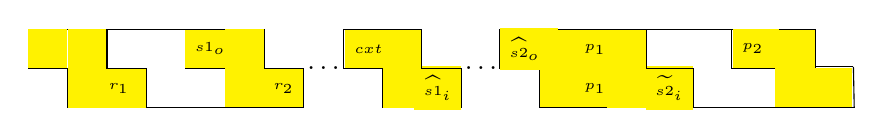
\begin{tikzpicture}
  \draw (0,1) -- (3,1) ;
  \draw (4,1) -- (5,1) ;
  \draw (0.5,0) -- (3.5,0);
  \draw (4.5,0) -- (5.5,0) ;
  \draw (0,1)--(0,0.5) -- (0.5,0.5) -- (0.5,0) -- (1.5,0) ;
  \draw (0.25,0.75)  node[minimum size=0.495cm,fill=yellow] {${ \silent}$};
  \draw (0.75,0.75)  node[minimum size=0.5cm,fill=yellow] {$\ $};
  \draw (0.76,0.25)  node[minimum size=0.5cm,fill=yellow] {$\ $};
  \draw (1.21,0.25)  node[minimum size=0.5cm,fill=yellow] {${\scriptscriptstyle r_1 \ }$};
 
  
  \draw (2,1) -- (2,0.5) -- (2.5,0.5) -- (2.5,0) -- (1.5,0)  -- (1.5,0.5) -- (1,0.5) -- (1,1);

 \draw (1.25,0.75) node{$\noact$};%node[minimum size=0.5cm,draw,draw=white] {$\noact$};
 \draw (2.25,0.25) node{$\noact$};
 \draw (2.31,0.75)  node[minimum size=0.47cm,draw,fill=yellow, draw=yellow] {${\scriptscriptstyle s1_o}$};
  \draw (2.75,0.75)  node[minimum size=0.48cm,draw,fill=yellow,yellow] {$\ $};
  \draw (2.75,0.26)  node[minimum size=0.49cm,draw,fill=yellow,yellow] {$\ $};

  \draw (3.245,0.25)  node[minimum size=0.475cm,draw,fill=yellow,draw=yellow] {${\scriptscriptstyle   r_2}$};
  
  \draw (3.75,0.5) node{$\dots$};
  
  \draw(3.5,0.5) -- (3.5,0);
%%     \draw (3.25,0.75)  node[minimum size=0.5cm,draw,draw=white] {$\noact$};
%%  \draw (3.75,0.75)  node[minimum size=0.5cm,draw,white] {$\ $};
%%  \draw (3.75,0.25)  node[minimum size=0.5cm,draw,white] {$\ $};
%%  \draw (4.25,0.25)  node[minimum size=0.5cm,draw,draw=white] {$\noact$};
\draw  (4,1) --  (4,0.5) -- (4.5,0.5) -- (4.5,0)   (3.5,0.5) -- (3,0.5) -- (3,1);
% \draw (3.25,0.75) node{$\noact$};%node[minimum size=0.5cm,draw,draw=white] {$\noact$};
%  \draw (4.25,0.25) node{$\noact$};
\draw (4.75,0.745)  node[minimum size=0.485cm,draw,fill=yellow,yellow] {$\ $};
  \draw (4.38,0.75) node[minimum size=0.47cm,draw,fill=yellow, draw=yellow] 
  {${\scriptscriptstyle  cxt \ }$};
  
  \draw (4.75,0.25)  node[minimum size=0.48cm,draw,fill=yellow,yellow] {$\ $};
  \draw (5.2,0.255)  node[minimum size=0.485cm,draw,fill=yellow,draw=yellow] {${\scriptscriptstyle  \widehat{s1}_i}$};
  \draw(5,1) -- (5,0.5) -- (5.5,0.5) -- (5.5,0);
   
   \draw (5.75,0.5) node{$\dots$};
   
    \draw (6,1) -- (10,1) ;
 %   \draw (7,1) -- (7,0.5) -- (7.5,0.5) -- (7.5,0);
    \draw (6.5,0) -- (10.5,0);
    \draw   (5.99,1)-- (5.99,0.5) -- (6.5,0.5) -- (6.5,0.5) -- (6.5,0) ;
    \
     \draw (6.75,0.75)  node[minimum size=0.47cm,fill=yellow, draw=yellow] {$\ $};
 \draw (6.36,0.75) node[minimum size=0.475cm,draw,fill=yellow,draw=yellow] 
 {${\scriptscriptstyle \widehat{s2}_o \ }$};
 %node[minimum size=0.5cm,draw,draw=white] {$\noact$};
   \draw (6.75,0.26)  node[minimum size=0.485cm,fill=yellow, draw=yellow] {$\ $};

% \draw (7.20,0.25) node[minimum size=0.475cm,fill=yellow, draw=yellow] {${\scriptscriptstyle{p_1}} \ 
\draw (7.20,0.25)  node[minimum size=0.475cm,draw,fill=yellow,draw=yellow] {${\scriptscriptstyle p_1}$};
\draw (7.2,0.74) node[minimum size=0.48cm,draw,fill=yellow,draw=yellow]{${\scriptscriptstyle p_1}$};
\draw (7.6,0.74)  node[minimum size=0.48cm,draw,fill=yellow, draw=yellow] {$ \ $};
\draw (7.6,0.25)  node[minimum size=0.48cm,draw,fill=yellow, draw=yellow] {$ \ $};
\draw (8.14,0.25)  node[minimum size=0.475cm,draw,fill=yellow,draw=yellow] {${\scriptscriptstyle \widetilde{s2}_i}$};
 \draw (8.14,0.75) node{$\noact$};%node[minimum size=0.5cm,draw,draw=white] {$\noact$};
 \draw (9.24,0.25) node{$\noact$};
  \draw (7.85,1) -- (7.85,0.5) ;
   \draw (7.85,0.5) -- (8.45,0.5) ;
      \draw  (8.45,0.5) --(8.45,0) ;
       \draw  (8.93,1) --(8.93,0.5) ;
        \draw  (8.93,0.5) --(9.5,0.5) ;
             \draw  (9.49,0.5) --(9.49,0) ;
         \draw  (9.49,0.5) --(9.49,0) ;
         \draw(10.0,1) -- (10.0,0.5);
          \draw(10,0.52) -- (10.48,0.52);
          \draw(10.48,0.52)--(10.49,0);
%  $};
%
%%     \draw (7.3,0.75)   node{$\noact$};
%%  \draw (7.75,0.75) node{$\ $};
%%  \draw (7.76,0.26) node {$\ $};
%%  \draw (8.25,0.26)  node {$\noact$ };
%
%  \draw (8.3,0.75)  node[minimum size=0.48cm,draw,fill=yellow, draw=yellow] {${\scriptscriptstyle \hat{s2}_o}$};
%  \draw (8,1)--(8,0.5)--(8.5,0.5) -- (8.5,0);
% % \draw(9.5,0.5) --(9.5,0);
%  \draw (8.745,0.75)  node[minimum size=0.48cm,draw,fill=yellow,yellow] {$\ $};
%  \draw (8.75,0.26)  node[minimum size=0.48cm,draw,fill=yellow,yellow] {$\ $};
 %\draw (9.24,0.26)  node[minimum size=0.48cm,draw,fill=yellow,draw=yellow] {${\scriptscriptstyle p_1}$};
 %\draw(9.5,0.5) --(9.5,0);
    % \draw (9,1) -- (10,1) -- (10,0.5) -- (10.5,0.5) --  (10.5,0) -- (9.5,0)  (9.5,0.5) -- (9,0.5) -- (9,1);
 \draw (9.24,0.75) node[minimum size=0.48cm,draw,fill=yellow,draw=yellow]{${\scriptscriptstyle p_2 \; }$};%node[minimum size=0.5cm,draw,draw=white] {$\noact$};
 
 \draw (10.22,0.26) node [minimum size=0.48cm,draw,fill=yellow,draw=yellow]{$\silent $};
%{${\scriptscriptstyle \tilde{s1}_i}$};
 \draw (9.74,0.745) node [minimum size=0.485cm,draw,fill=yellow,draw=yellow]{$\ $};
 \draw (9.735,0.26) node [minimum size=0.48cm,draw,fill=yellow,draw=yellow]{$\ $};
 %  \draw (10.8,0.5) node{$\dots$};
% \draw (10,1) -- (10,0.5) -- (10.5,0.5)--(10.5,0);
  %\draw (10.31,0.75)  node{$\noact$};
%  \draw (10.75,0.75)  node {$\ $};
%  \draw (10.75,0.26)  node{$\ $};
% \draw (11.25,0.25)  node {$\noact$};
%   \draw (11,1) -- (11,0.5) -- (11.5,0.5) -- (11.5,0);% -- (10,0) -- (9,0) -- (9,0.5) -- (8.5,0.5) -- (8.5,1);
%    \draw (11,1) -- (11.5,1) -- (12,1) -- (12,0.5) -- (12.5,0.5)--(12.5,0)--(11.5,0);
   %\draw (11.25,0.25)  node[minimum size=0.48cm,draw,fill=yellow,draw=yellow] {$\noact$};
%    \draw (11.31,0.75) node[minimum size=0.48cm,draw,fill=yellow,draw=yellow]{${\scriptscriptstyle \tilde{s1}_o}$};
%    \draw (11.75,0.26)node[minimum size=0.48cm,draw,fill=yellow,draw=yellow]{$\ $};
%      \draw (11.75,0.75)node[minimum size=0.48cm,draw,fill=yellow,draw=yellow]{$\ $};
%     \draw (12.2,0.25) node[minimum size=0.478cm,draw,fill=yellow,draw=yellow]{\;$\silent$\;  };
  \end{tikzpicture}
  $
  \underbrace{\phantom{loremipsu}}_\text{Init}   \underbrace{\phantom{loremipsuo}}_\text{$P_{r1} (P_{s1})$} \underbrace{\phantom{loremip}}_\text{ $P_{r2}(\overline{P}_{s2})$}\underbrace{\phantom{loremipsumlore}}_\text{$Cxt (P_{s1},\overline{P}_{s2})$}
     \underbrace{\phantom{loremipsumlo}}_\text{$P_{r1} (\overline{P}_{s2})$}
      \underbrace{\phantom{loremip}}_\text{ $P_{r2}$}
  $
  \caption{The link chain structure arising from reactions and context processes.}
   \label{fig:backbone}
 \end{figure}
 \end{example}

Example~\ref{ex:backbone}   outlines two different roles of the processes defining the translation of an interactive process: those processes encoding the reactions and the context provide the backbone of each transition, whereas the processes encoding the entities provide the resources needed for the communication to take place.

\paragraph{The flat function}
For technical reasons, our transition labels are quite verbose; then, to simplify their processing, we introduce a function that takes a solid link chain and returns a simple string by eliminating all the channel matching pairs leaving just one placeholder for them. This transformation is harmless, in the sense that it retains all the information in the chain, because it is applied to complete chains only. 
The function $\mathit{flat}(\cdot)$ is defined inductively as follows:
%\[
%\begin{array}{lcl@{\hspace{0.5cm}}lcl@{\hspace{0.5cm}}lcl@{\hspace{0.5cm}}lcl}
%\mathit{flat}(\epsilon)&\defeq & \epsilon &
%\mathit{flat}(\link{\gamma}{\gamma'}) &  \defeq & \left \{ \begin{array}{cl} \epsilon & \mathrm{if } (\gamma = \beta_i \wedge \gamma = \beta_o)  \vee \gamma = \silent\\
%\gamma' & \mathrm{otw }  \end{array} \right. &
%%\mathit{flat}(\link{\alpha}{\silent})& \defeq & \epsilon &
%%\mathit{flat}(\link{\alpha}{\beta}) & \defeq &\beta \\
%\end{array}\]

\[
\mathit{flat}(\epsilon)\defeq \epsilon 
\qquad
\mathit{flat}(\link{\alpha}{\beta}) \defeq 
\left \{ \begin{array}{ll} 
\beta & \mbox{if $\beta\in \mathit{reacts}\cup\{\mathit{cxt}\}\cup\mathit{prods}$}\\
d & \mbox{if $\beta=d_i$ with $d\in\mathit{decs}$}\\
\epsilon & \mbox{otherwise}  
\end{array} \right. 
\]

\[
\begin{array}{lcl}
\mathit{flat}(\link{\alpha}{\beta}\upsilon)& \defeq & \mathit{flat}(\link{\alpha}{\beta}) \mathit{flat}(\upsilon)\\
\end{array}\\
\]
{\color{red} where the juxtaposition of two string results in the   
%$::$ is the 
usual string concatenation operator.}

For example, if we consider again the complete label
$$
\upsilon =  \startchain{\silent}
 \chainedlink{r_1}{r_1}
 \chainedlink{s1_i}{s1_i}
 \chainedlink{s1_o}{s1_o}
 \chainedlink{r_2}{r_2}
 \chainedlink{\overline{s2}_i}{\overline{s2}_i}
 \chainedlink{\overline{s2}_o}{\overline{s2}_o}
 \chainedlink{\mathit{cxt}}{\mathit{cxt}}
 \chainedlink{\widehat{s1}_i}{\widehat{s1}_i}
 \chainedlink{\widehat{s1}_o}{\widehat{s1}_o}
  \chainedlink{\widehat{s2}_i}{\widehat{s2}_i}
  \chainedlink{\widehat{s2}_o}{\widehat{s2}_o}
  \chainedlink{p_1}{p_1}
  \chainedlink{\widetilde{s2}_i}{\widetilde{s2}_i}
  \chainedlink{\widetilde{s2}_o}{\widetilde{s2}_o}
  \chainedlink{p_2}{p_2}
  \chainend{\silent}
$$
from Example~\ref{ex:backbone}, we have
$$
\mathit{flat}(\upsilon) = 
r_1\ 
s1\ 
r_2\
\overline{s2}\ 
\mathit{cxt}\ 
\widehat{s1}\ 
\widehat{s2}\ 
p_1\ 
\widetilde{s2}\ 
p_2.
$$

It is then immediate to define the function $\mathit{unflat}$ to rebuild the complete label from the compact string (here we exploit again the half link and block notation):
$$
\mathit{unflat}(x) \defeq\left\{
\begin{array}{ll}
^{x}_{x} & \mbox{if $x\in \mathit{reacts}\cup\{\mathit{cxt}\}\cup\mathit{prods}$}\\
^{x_i}_{x_i}\backslash^{x_o}_{x_o} & \mbox{if $x\in \mathit{decs}$}\\
\end{array}
\right.
$$
$$
\mathit{unflat}(x_1\dots x_n) \defeq\ ^{\silent}\backslash \mathit{unflat}(x_1) \backslash \dots \backslash \mathit{unflat}(x_n) \backslash_{\silent}
$$

It is immediate to check that for any complete label $\upsilon$ of our processes we have
$\upsilon = \mathit{unflat}(\mathit{flat}(\upsilon))$.


With the next proposition, we analyse the structure of a c\CNA \ 
process encoding of  a reactive process after one transition step.
In the following four statements, for brevity, we let ${\cal A} = (S, A)$ be a RS, and let  $\pi=(\gamma,\delta)$ be an extended interactive process in $A$, with $\gamma=\{C_i\}_{i\in\mathbb{N}}$ and $\delta=\{D_i\}_{i\in\mathbb{N}}$. 

 \begin{restatable}[Correctness 1]{proposition}{propcorruno}
% \begin{proposition}(correctness 1)\\
 \label{prop:corr1}
% We define $\pi' = (\gamma',\delta')$ with $\gamma' = C_0',\dots,C_{n-1}'$ and $\delta' = D_0',\dots,D_{n-1}'$ as $C_0' = C_1 \cup D_1$,  and
% $C_i' = C_{i+1}$, $D_{i}' = D_{i+1}$ with $ 1 \leq i < n$.
 Let 
 $P=\llbracket{\cal A},\gamma\rrbracket$ with
$$P  = \restrict{\mathit{names}} \left(I~|~\prod_{a \in A}P_a ~|~ \mathit{Cxt}^1 ~|~ \prod_{s \in C_0}P_s ~|~ \prod_{s \notin C_0}\overline{P}_s\right).
$$
 If there exists  $P'$  such that $P \xrightarrow{v}P'$,  it holds that:
 \begin{enumerate}
 \item
  $v=\link{\silent}{\silent}\dots\link{\silent}{\silent}$, and
  \item 
 $P'= \restrict{\mathit{names}} \left(I~|~\prod_{a \in A}P_a~|~ \mathit{Cxt}^2 ~|~ \prod_{s \in C_1 \cup D_1}P_s| \prod_{s \notin C_1 \cup D_1}\overline{P}_s\right)$.
 \end{enumerate}
Moreover, given $\pi^1=(\gamma^1,\delta^1)$, we have $P' = \llbracket {\cal A},\gamma^1\rrbracket$.
 %\end{proposition}
\end{restatable}
 
% \begin{lemma}[correctness 1 {\color{red} Ma serve ??}]
% \label{cor:complet1}
% Let ${\cal A} = (S, A)$ be a rs, and let  $\pi=(\gamma,\delta)$ be an extended interactive process in $A$, with
% $\gamma = C_0,\dots,C_t$, $\delta = D_0,\dots,D_t$, with $n \geq 0$. Let   $P=[|{\cal A},\gamma|]$ be  its c\CNA~translation. We define $\pi' = (\gamma',\delta')$ with $\gamma' = C_0',\dots,C_{n-1}'$ and $\delta' = D_0',\dots,D_{n-1}'$ as $C_0' = C_1 \cup D_1$,  and
% $C_i' = C_{i+1}$, $D_{i}' = D_{i+1}$ with $ 1 \leq i < n$. Then,
% if $\exists$ $P'$, $P''$ such that $P \xrightarrow{\link{\silent}{\silent}} P'$ and $P \xrightarrow{\link{\silent}{\silent}} P''$, then $P' = P''$.
%\end{lemma}

 
 
% \begin{proposition}[correctness2]
% \label{prop:correctness1}
% Let $P$ be a c\CNA \ process such that $\exists$ a $rs$ ${\cal A}$ and a $n$-step interactive process $\pi=(\gamma,\delta)$ with $\gamma =C_0,\dots,C_n$ and $\delta = D_0,\dots,D_n$ such that $P= [|{\cal A},\gamma|]$. 
% %We set $\pi'=(\gamma',\delta')$ with $\gamma'=C_0',\dots,C_{n-1}'$,  $\delta'=D_0',\dots,D_{n-1}$,  where $C_0'= C_1 \cup D_1$, $C_i'= C_{i+1}$, $D_i=D_{i+1}'$,  and $1 \leq i < n$.
%Then,   $\exists$ $P'$ and $\pi'=(\gamma',\delta')$ such that $P \xrightarrow{\link{\silent}{\silent}}P'$, $P' =[|{\cal A},\gamma'|]$.
% \end{proposition} 

Now, we extend the previous result to a series of transitions.
 
 \begin{restatable}[Correctness 2]{corollary}{corrcorrdue} 
% \begin{corollary}[correcteness2]
 \label{corr:corr2}
  Let $P = \llbracket{\cal A},\gamma\rrbracket$ and $j\geq 1$.
%  Let $P$ a  c\CNA process such that exists a rs ${\cal A}$ and an extended  interactive process $\pi=(\gamma,\delta)$ with $\gamma =C_0,\dots,C_t$, $\delta = D_0,\dots,D_t$, with $t \geq 0$, such that $P= [|{\cal A},\gamma|]$. 
If there exists  $P''$ such that $P \xrightarrow{\link{\silent}{\silent}\dots \link{\silent}{\silent}}^{j}P''$, then letting  $\pi^j=(\gamma^j,\delta^j)$ we have
$P'' =\llbracket{\cal A},\gamma^j\rrbracket$.
%such that $P=[|{\cal A}|]$, then if $P \rightarrow^* P'$, then $\exists$ ${\cal A'}$ such that ${\cal A}$  evolves in ${\cal A'}$ and $P'=[|{\cal A'}|]$.
 \end{restatable}


With the following propositions, we prove that, given a RS ${\cal A} = (S, A)$ and an extended  interactive process $\pi=(\gamma,\delta)$, then the $c\CNA$ process $\llbracket{\cal A},\gamma\rrbracket$ can simulate all the evolutions  of $\pi$. 

 \begin{restatable}[Completeness 1]{proposition}{propcompluno} 
% \begin{corollary}[correcteness2]
 \label{prop:compl1}
% \begin{proposition}[completeness1]
 %\label{lem:compl2}
Let   $P=\llbracket{\cal A},\gamma\rrbracket$ and $\pi^1 = (\gamma^1,\delta^1)$.
% be the extended interactive process starting  at the next state sequence. 
Then, 
 % following holds:
 %\begin{enumerate} 
 %\item  
  $P \xrightarrow{\link{\silent}{\silent}\dots \link{\silent}{\silent}} P'=\llbracket{\cal A},\gamma^1\rrbracket$.
 %\item if $\exists$ $P'$, $P''$ such that $P \xrightarrow{\link{\silent}{\silent}} P'$ and $P \xrightarrow{\link{\silent}{\silent}} P''$, then $P' = P''$.
 %\end{enumerate}
% \end{proposition} 
\end{restatable}


Now, we extend the previous result to a series of transitions.
 
\begin{restatable}[Completeness 2]{corollary}{corrcompldue} 
% \begin{corollary}[correcteness2]
 \label{corr:compl2}
% \begin{corollary}[completeness2]
 %\label{prop:completeness}
Let $P=\llbracket{\cal A},\gamma\rrbracket$ and  $\pi^j= (\gamma^j,\delta^j)$.  
Then, $P \xrightarrow{\link{\silent}{\silent}\dots\link{\silent}{\silent}}^j P''=\llbracket{\cal A},\gamma^j\rrbracket$.  
 \end{restatable}




 
% 
% \begin{proposition}[correctness]
% Let $P$ a c\CNA\  process such that exists a reaction system ${\cal A}$ such that $P=[|{\cal A}|]$, then if $P \rightarrow P'$, then $\exists$ ${\cal A'}$ such that ${\cal A}$  evolves in ${\cal A'}$ in one step and $P'=[|{\cal A'}|]$.
% \end{proposition}
 
 
 
 
  